\documentclass[12pt]{article}
\usepackage{graphicx}
\begin{document}

\begin{titlepage}
\centerline{Data Collection Concept Addressing Food Inefficiency in The Upcountry Regions of Uganda\\}
\paragraph*{•}
\centerline{ KONGORO DICKENS 16/U/18805 216020616.\\}
\centerline{ Makerere University Feb 23, 2018\\}
\paragraph*{•}
\paragraph*{•}
\end{titlepage}
\newpage
\section{Introduction}
\paragraph{•}There has been a massive increase in food insufficiency in the upcountry regions of Uganda over the past five years and there is every indication that this will continue if solutions are not effectively implemented. According to FAO (Food Agriculture Organization 2007) by 2020 almost 80$\%$ of people in leaving in Upcountry  regions will be have a single meal each day. FAO describes this phenomenon as ‘serious in the extreme, potentially undermining the the growth and development in a society’ (2007, p 167). Currently in Karamoja about 100 people die in six months.
Recently the representatives at the Ugandan parliament  complained about the ignorance and less care the government is showing them.  At present there is no policy regarding the measures that can help put things back to order.
\section{Data to be collected}
\paragraph{•}Apart from food insufficiency and the number of acres of land that the people in the upcountry regions of Uganda do cultivate, more data such us level of education, number of family members, methods of food storage and the main purpose for food growth which may also be a leading factor to this problem in the Upcountry regions of Uganda.
\paragraph{}More so from the questionnaire conducted it has been brought to light that poor food storage of the food is the leading cause of food insufficiency in those areas. And also, the level of education also is a highly determining factor to food insecurity which to a larger extent cause insufficiency. 
\newpage
\begin{figure}
  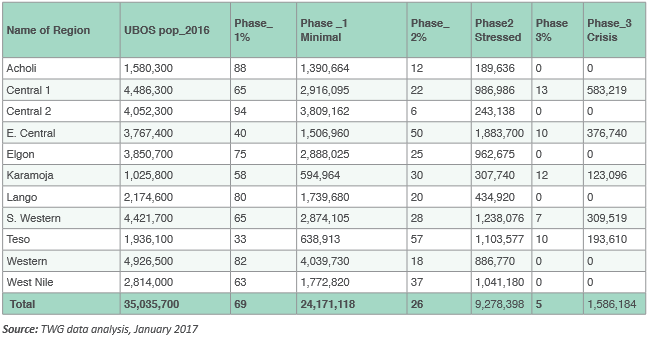
\includegraphics[width=\linewidth]{Food.png}
  \caption{Tables showing Population in the Upcountry Regions And food consumption}
  \label{fig:Table1}
\end{figure}
\end{document}